\documentclass[a4paper]{article}
\usepackage{graphicx}
\usepackage{url}
%\usepackage{onecolpceurws}

\title{New Approach To Find The Origins Of a Bug }

\author{
Gema Rodriguez-Perez \\ LibreSoft/GSyC\\
                Universidad Rey Juan Carlos \\ gerope@libresoft.info
\and
Gregorio Robles \\ LibreSoft/GSyC\\
                Universidad Rey Juan Carlos \\ grex@gsyc.urjc.es
\and
Jesus M. Gonzalez-Barahona \\LibreSoft/GSyC\\
                Universidad Rey Juan Carlos \\ jgb@gsyc.est
}


\begin{document}
\maketitle

\begin{abstract}

This paper presents our ongoing research work. The core of our study is focused on bug fixing and bug seeding process, concretely, in the study of the assumption made in the literature which says that a given bug was introduced by the lines of code that were modified to fix it. After exploring carefully how a number of bugs were introduced in two different projects, we have developed an approach of how bugs are introduced. Furthermore, based on the above assumption we are carrying out a systematic review about the use of this assumption in previous research works.

\end{abstract}


\section{How to locate the origin of a bug: The SZZ algorithm}

To fix a bug in a software it seems necessary to understand why it is behaving erroneously, and then modify the source code that is causing such behaviour producing a change to the code identified as the bug-fixing change. Thanks to the modern software development projects, we have many information at our disposal that allows us identify where exactly a bug-fixing change was done. However, identify the previous change(s) responsible to cause the bug that was later fixed is not a trivial task and it could be a very interesting exercise.

The problem of locating the change causing a bug has already been addressed in previous work. Silwerski, Zimmermann, and Zeller were successfully able to identify changes in version control that induced fixes of bugs creating the well-known algorithm SZZ~\cite{sliwerski2005changes}. The main assumption of this algorithm is base on the idea that modified or removed lines in a fixing-commit are the ones suspicious of inducing the later fix. Thus, tracing back them in the source code management system to the time when they were modified or added result in the commit that is considered as the cause of the bug.

However, we know that exists certain common change patterns that occur in the normal development process that make this method less useful, such as an older modification, or a change in some API in a different part of the code. Thus, this causes issues when you attempt to identify the location of the bug by assuming that the last modification to change that particular line has injected the buggy line.

\subsection{Credibility of the SZZ algorithm}

Since the publication of the SZZ algorithm, adaptations of this algorithm have been described in many studies, causing that such algorithm has become a standard for bug prediction and bug detection studies.

For example, Prechelt and Pepper described in detail the limitations of the methods to identify the bug inducing change when adopted by practitioners~\cite{prechelt2014software}. German \emph{et al.}~\cite{german2009change} noticed that software is continuously changing and as result, changes might have impact across the whole system causing that the bug may be located in a different part from the source of the bug.

Also, Hata \emph{et al.} introduces an approach for fault-prone module detection. Using the SZZ to  identify the faulty modules in spite of their knowledge of some limitations~\cite{hata2010fault}. In the same line, Mizuno \emph{et al.} proposes a model that predict the likelihood that a change will be a bug inducing commit based on the use of SZZ to identify faulty modules, despite the limitations they described in their paper~\cite{mizuno2010prediction}.

Furthermore, in a recent study by Da Costa \emph{et al.} the results of five alternative SZZ implementations have been evaluated using a proposed a framework. The results point out that the current SZZ implementations still lack mechanisms to correctly identify the \emph{real} bug inducing commits. In addition, they describe some of the main problems that are not addressed by SZZ as well as how SZZ may flag potential bug inducing changes that were correct at the time of committing~\cite{da2016framework}.

The limitations of the SZZ algorithm are known as the previous paragraphs have showed, but researchers are still using it in their studies. Currently the SZZ algorithm paper has more than 500 cites, to understand how and why researchers have used it, we are working on a systematic review of previous studies that have used this algorithm, with a specific focus on the purpose, methods, and credibility. The review uses more than 400 papers in journals, conference proceedings, workshops and thesis publications. The main goal of this work is to better understand how others use this algorithm and also provide some guidelines to improve the credibility of techniques that are used to locate the origins of the bug.

\section{New approach to find the origins of a bug}

To mitigate the false positives that such algorithm causes, we believe in the idea that version control system bisection provides. Hence an issue is resolved and a test case is added in a revision, we might know that the bug have been injected before that revision. Thus, going back to previous revisions and testing the software we might determine whether or not the bug is present. If it is indeed present, the test case fails and the bug must have been injected before (or by) that revision. In our work and base on this idea, we have used information from the source code management system, the issue tracking system and the code review system to first understand which was the malfunction caused by the bug, what problems in the source code were causing it, and how it was finally fixed. Furthermore, we have used all the history of the software component, to find out the moment when the malfunction happened for the first time, and which change(s) to the code, introduced it. 

Figure~\ref{fig:test} shows the check test idea. We are able to find the suspicious commit to be the bug inducing commit based on the idea of having an omnipotent view. Thus, the test is passed to all previous commits looking for the one that fails; if found, we will be consider it as a candidate for the bug inducing change.

\begin{figure}[ht]
\centering
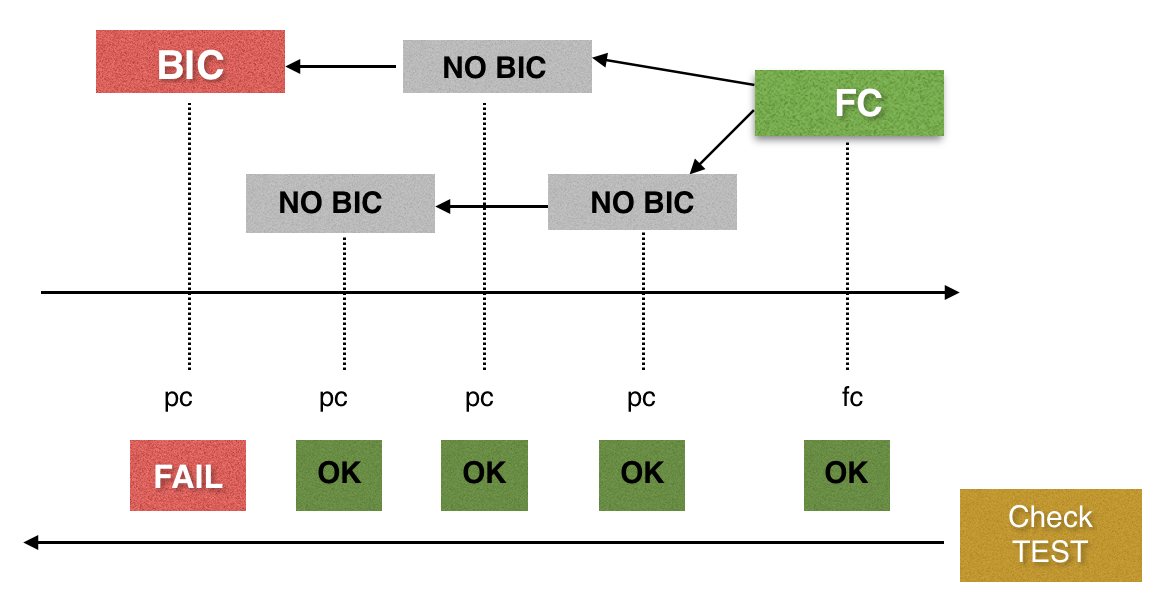
\includegraphics[width=\columnwidth]{testrecursive.png}
\caption{Example of how we could find a candidate commit to be the  bug inducing change. Each version passes or not a test written after fixing the bug in the FC (fixing commit).}
\label{fig:test}      
\end{figure}

Next, the methodology that we have used in our empirical experiment to find the origin of the malfunction in the software using a method based on lines and a method based on tokens is described. In the case of Nova and ElasticSearch, the data needed can be obtained from the source code management, issue tracking system, and code review system. 

Figure~\ref{fig:diagram} provides an overview of each step involved in our study and their outcomes.

\begin{figure}[ht]
\centering
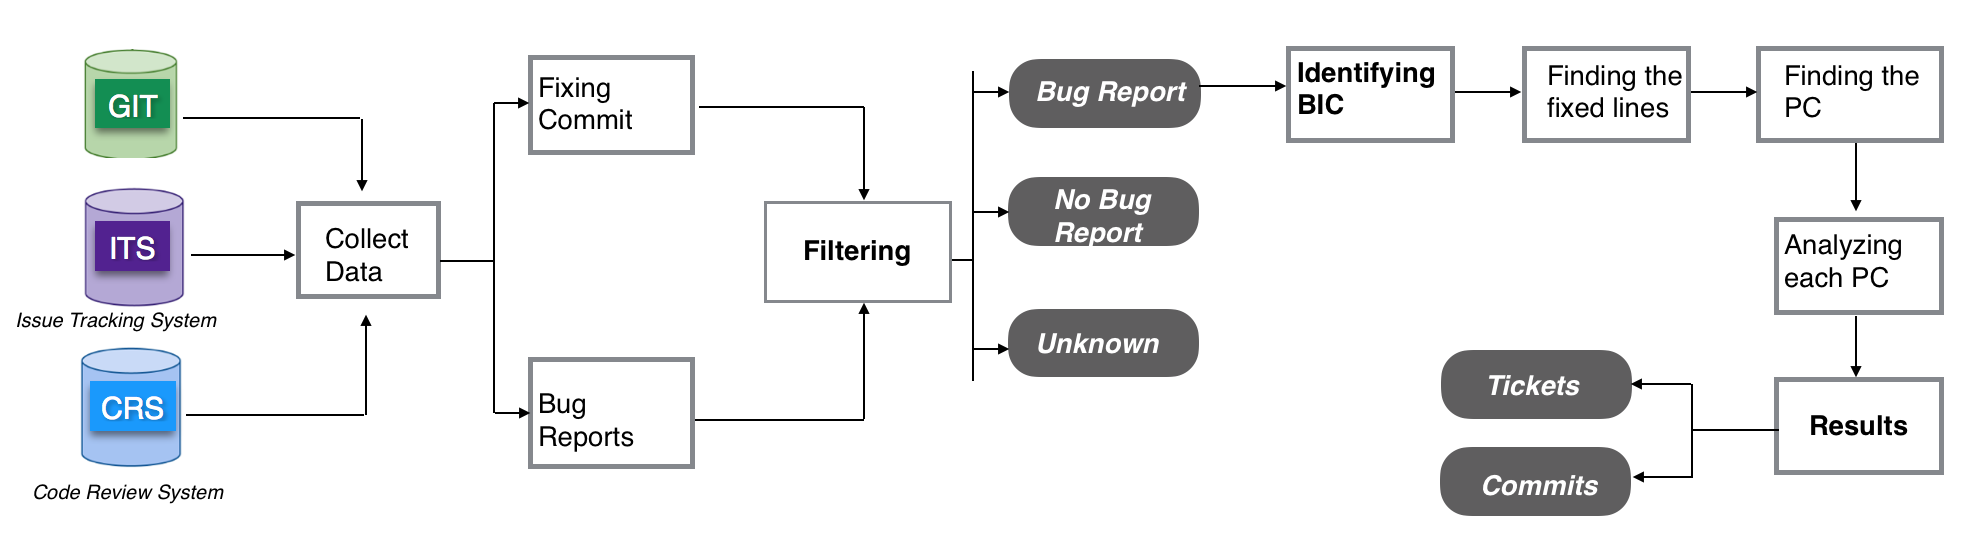
\includegraphics[width=\columnwidth]{diagram.png}
\caption{Overview of the steps involved in our analysis. \emph{PC} refers to the immediately previous commit of a fixed line }
\label{fig:diagram}       % Give a unique label
\end{figure}

At the end of this step we have two main groups for each bug analyzed:
\begin{itemize}
	\item Group 1 : The bug has been always there, then the test will always fail.
	\item Group 2: The bug can be found using the test. Thus, we have two main reasons: (a) The test fails as we expected because the failure was due to a change in other part of the code that affects the code fixed or  the fixed line(s)/token(s) cannot be checked before because they didn't exists. (b) The test fails because a previous change (the $pc$ or an older commit) injected the bug.
\end{itemize}

\subsubsection{New Metrics}

Furthermore, once we know exactly the moment of the malfunction we are able to calculate metrics such as the Time To Fix (TTF), the Time To Review (TTR), the Time To Notify (TTN) a bug or the fix-effort to improve code quality and to study the relationship between them that may prevent the injection of bugs in the future.

Figure~\ref{fig:metrics} provides a visual explanation of the metrics that we propose. For example, to obtain the metrics for bug report, we need to identify the fixing commit and the bug inducing change. Then, analyzing the meta-data of theses commits, we obtain the date and the author for both of them.

\begin{figure}[ht]
\centering
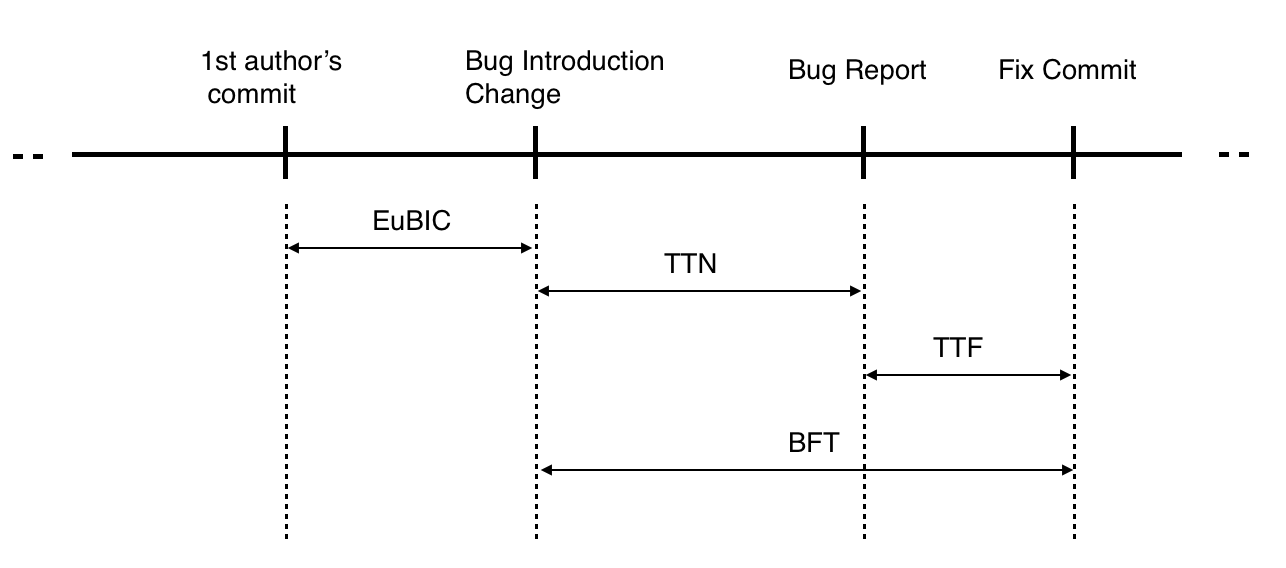
\includegraphics[width=\columnwidth]{metrics.png}
\caption{Visualization of the periods under study: Experience Until Bug Introducing Change (EuBIC),  Time To Notify (TTN), Time To Fix (TTF), Bug Fixing Time (BFT).}
\label{fig:metrics}       % Give a unique label
\end{figure}

\paragraph{Experience until Bug Introducing Change (EuBIC):}
Experience measures in days of the author inserting the bug at the moment of doing the commit. 
\paragraph{Time To Notify (TTN):}
Time in days since the bug inducing commit was merged into the master branch until some developer notified the bug and reported it in the bug tracking system. 
\paragraph{Time To Fix (TTF):}
Period in days from the notification of a bug report to when it was closed with a fixing commit.
\paragraph{Bug Fixing Time (BFT):}
Time in days from the date of the bug inducing change to the fixing commit date.

\section{Conclusions and further research}

In this paper we present two of our ongoing research works, the first describes a new approach to locate the origin of a bug base on the idea of testing each previous version until find the version that causes the malfunction of the code. This way, we could reduce the false positives and also find the missing false negatives that other approach give us. And this empirical study gives cause for understanding how metrics extracted from the precise location of a bug are related to the maintenance and evolution of a software.

While the second one provides deep insight on the credibility of the most known algorithm to locate the line(s) that injected the bug into the source code. With a systematic review of this algorithm we try to understand how other studies used it and what was their purpose.

A future line could be the full automation of the methodology used in this paper, that would provide software projects with a valuable tool for understanding how bugs are introduced, and therefore calculate these metrics for mitigation.

\begin{thebibliography}{Com79}

\bibitem[sliwerski2005]{sliwerski2005changes}
{\'S}liwerski, Jacek and Zimmermann, Thomas and Zeller, Andreas
\newblock When do changes induce fixes?.
\newblock {\em Proceedings of the 2005 International Workshop on Mining software repositories}, 1--5, 2005.

\bibitem[prechelt2014]{prechelt2014software}
Prechelt, Lutz and Pepper, Alexander.
\newblock {\em Why software repositories are not used for defect-insertion circumstance analysis more often: A case study -- Volume 56, 1377--1389 / Information and Software Technology}.
\newblock Elsevier, 2014.

\bibitem[german2009]{german2009change}
German, Daniel M and Hassan, Ahmed E and Robles, Gregorio
\newblock {\em Change impact graphs: Determining the impact of prior codechanges -- Volume 51, 1394--1408 / Information and Software Technology}.
\newblock Elsevier, 2009.

\bibitem[hata2010]{hata2010fault}
Hata, Hideaki and Mizuno, Osamu and Kikuno, Tohru
\newblock {\em Fault-prone module detection using large-scale text features based on spam filtering -- Volume 15, 147--165 / Empirical Software Engineering}.
\newblock Springer, 2010.

\bibitem[mizuno2010]{mizuno2010prediction}
Mizuno, Osamu and Hata, Hideaki
\newblock {\em Prediction of fault-prone modules using a text filtering based metric -- Volume 4, 43--52 / International Journal of Software Engineering and Its Applications}.
\newblock 2010.

\bibitem[da2016]{da2016framework}
da Costa, Daniel Alencar and McIntosh, Shane and Shang, Weiyi and Kulesza, Uira and Coelho, Roberta and Hassan, Ahmed
\newblock {\em A Framework for Evaluating the Results of the {SZZ} Approach for Identifying Bug-Introducing Changes / IEEE Transactions on Software Engineering}.
\newblock IEEE, 2016.


\end{thebibliography}

\end{document}


